\section{Problemstellung}
In der HF-Technik kommt es sehr oft zur Situation, in welcher zwei Komponenten miteinander verbunden werden. Dieses auf den ersten Blick simple Vorhaben, kann einige Probleme bereiten. Haben die Komponenten unterschiedliche Impedanzen, spricht man von Fehlanpassung und es treten unerwünschte Reflexionen in der Leitung auf. Diese führen zu Verlusten und Verzerrungen des Signals. In diesem Bericht wird nun folgende Ausgangslage genauer betrachtet:
\begin{figure}[h]
	\centering
	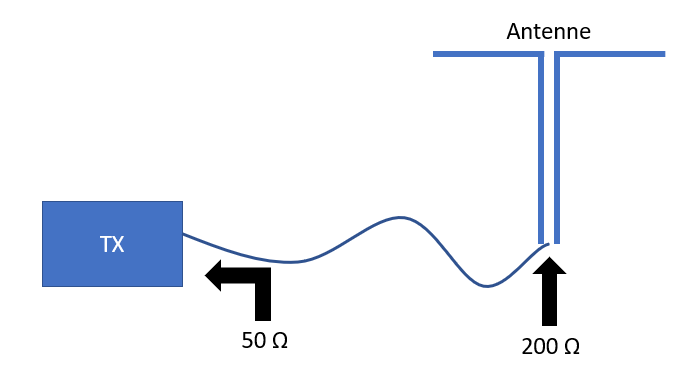
\includegraphics[width=0.6\linewidth]{ausgangslage.png}
	\caption{Ausgangslage Quelle an Antenne}\label{fig:ausgangslage}
\end{figure}

Eine 50$\Omega$-Quelle wird an eine 200$\Omega$-Dipol-Antenne mit einer Arbeitsfrequenz von \SI{20}{MHz} angeschlossen. Schliesst man die Antenne direkt an die Quelle wie in Abbildung \ref{fig:ausgangslage}, kommt es zur Fehlanpassung und den erwähnten Effekten. Die Impedanzanpassung ist jedoch nicht die einzige Herausforderung dieser Konstellation.
\newline
Weil nur die wenigsten Dipol-Antennen symmetrisch sind, fliessen Gleichtakt-Ausgleichsströme auf dem Aussenmantel der Leitung. Dadurch strahlt die Leitung ab und empfängt Störungen. Um diesen Sachverhalt genauer zu verstehen, betrachten wir zuerst eine ideale Dipol-Antenne.

\begin{figure}[H]
	\centering
	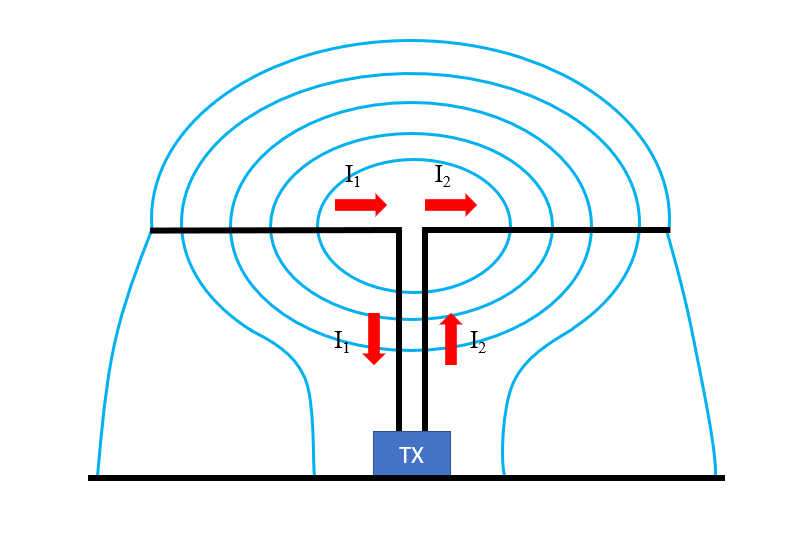
\includegraphics[width=0.8\linewidth]{idealer_dipol.png}
	\caption{Ströme und Felder bei einer idealen Dipol-Antenne}\label{fig:idealer_dipol}
\end{figure}

Sind beide Dipoläste exakt symmetrisch, sind die Impedanzen der einzelnen Äste gleich. Damit gilt für die Ströme $I_{1}=-I_{2}$. Sind die Ströme im Kabel Betragsgleich und entgegengesetzt, heben sich die Felder auf und die Leitung strahlt nicht ab.

Abbildung \ref{fig:realer_dipol} zeigt zum Vergleich die Felder wie sie in der Realität auftreten.
\begin{figure}[H]
	\centering
	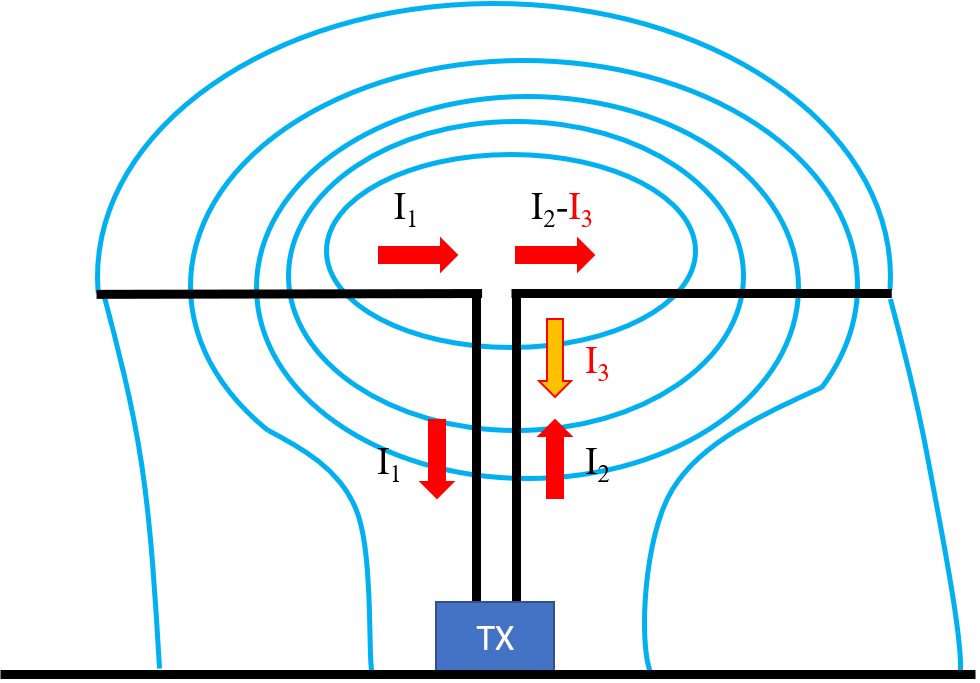
\includegraphics[width=0.8\linewidth]{realer_dipol.png}
	\caption{Ströme und Felder bei einer realen Dipol-Antenne}\label{fig:realer_dipol}
\end{figure}

Durch die Potentialunterschiede der Dipoläste kommt es zu Gleichtakt-Ausgleichsströmen auf der Speiseleitung. Die Leitung selber strahlt dadurch ab und wirkt als Antenne. \\

Das Ziel dieses Berichts liegt nun darin, einen Guanella-Balun, welcher die Impedanzanpassung und die Gleichtatkstromunterdrückung vornimmt, zu dimensionieren und zu realisieren.